\documentclass{article}
\newsavebox{\oldepsilon}
\savebox{\oldepsilon}{\ensuremath{\epsilon}}
\usepackage[minionint,mathlf,textlf]{MinionPro} % To gussy up a bit
\renewcommand*{\epsilon}{\usebox{\oldepsilon}}
\usepackage[margin=1in]{geometry}
\usepackage{graphicx} % For .eps inclusion
%\usepackage{indentfirst} % Controls indentation
\usepackage[compact]{titlesec} % For regulating spacing before section titles
\usepackage{adjustbox} % For vertically-aligned side-by-side minipages
\usepackage{array, amsmath,  mhchem}
\usepackage[hidelinks]{hyperref}
\usepackage{courier, subcaption}
\usepackage{multirow, enumerate}
\usepackage[autolinebreaks,framed,numbered]{mcode}

\usepackage{float}
\restylefloat{table}

\pagenumbering{gobble} 
\setlength\parindent{0 cm}
\renewcommand{\arraystretch}{1.2}
\begin{document}
\large

MCB 135 Problem Set 5 \hfill Due Monday, March 9, 2015 at 2:30 PM

\section*{Problem 1: Working with proteomics data (50 points)}

In this problem, you will explore the protein-protein interaction network recently described by \linebreak \href{http://www.cell.com/abstract/S0092-8674\%2814\%2901422-6}{Rolland et al. (2014)}. The interactions are provided in tab-delimited format on the course \linebreak website (\mcode{rolland.tsv}). Each line describes one interaction: the two columns give the \href{http://www.ncbi.nlm.nih.gov/gene}{NCBI \linebreak Entrez gene identification numbers} for the two proteins participating in the interaction.

\begin{enumerate}[a)]
\setlength{\itemsep}{0pt}
\item Determine the number of interactions in which each protein participates. (The MATLAB \linebreak functions \mcode{unique()} and \mcode{histcounts()} may be useful.)  Find the average number of interactions per protein, $\mu$.\\

\begin{lstlisting}
% Import data (copying and pasting also fine)
fid = fopen('rolland.tsv');
temp = textscan(fid, '%d\t%d');
data = [temp{1}, temp{2}];
fclose(fid);

protein_ids = unique(data);
interaction_counts = zeros(size(protein_ids));
self_interactions = 0;

for i=1:length(data(:,1))
    j = find(protein_ids == data(i,1));
    k = find(protein_ids == data(i,2));
    interaction_counts(j) = interaction_counts(j) + 1;
    if j == k
        self_interactions = self_interactions + 1;
    else
        interaction_counts(k) = interaction_counts(k) + 1;
    end
end

mu = mean(interaction_counts);
disp(sprintf('mu=%0.4f',mu));
\end{lstlisting}

{\color{red}
We found that $\mu \approx 6.36$.
}
\item Plot the distribution of interactions per protein -- i.e., the probability that a randomly-chosen protein participates in $x$ interactions -- on log-log axes.\\

\begin{lstlisting}
% Now we tally the number of proteins with each number of interactions
maximum_number_of_counts = max(interaction_counts);
x = 1:maximum_number_of_counts+1;
y = histcounts(interaction_counts, x) ./ (length(protein_ids));
x = x(1:length(x)-1);

% Plot the distribution of edge counts for the real data.
plot(x,y,'-k'); hold on;
axis([1 300 1e-6 1])
legend('Data','Location','NorthEast')
set(gca,'XScale','log','YScale','log','FontSize',16)
xlabel('Number of interactions')
ylabel('Frequency')
\end{lstlisting}

\begin{center}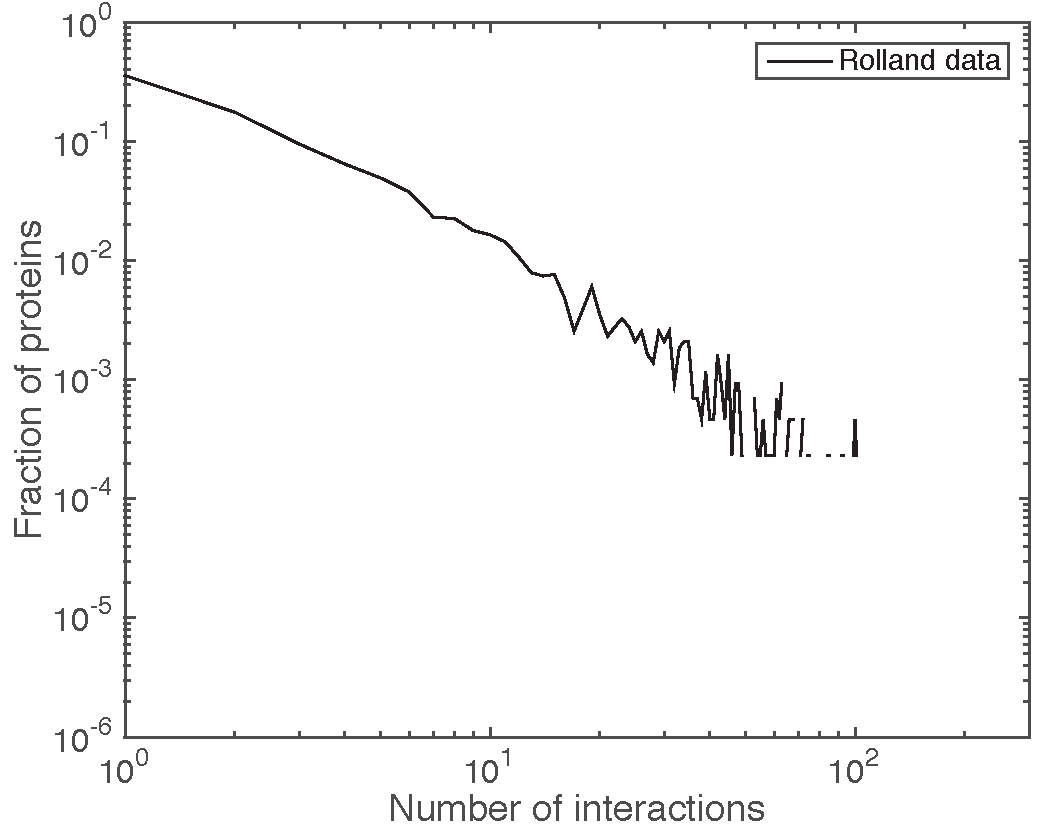
\includegraphics[width=0.4 \textwidth]{prob2b.pdf}\end{center}

\end{enumerate}
Under the hypothesis that all possible edges in a network occur with equal probability, the number of edges per node is expected to follow a Poisson distribution. 
\begin{enumerate}[a)]
\setlength{\itemsep}{0pt}
\setcounter{enumi}{2}
\item Plot a Poisson distribution with parameter $\mu$ on the same axes as the true distribution of interaction counts. In MATLAB, this can be done with the function \mcode{poisspdf()}.\\

\begin{lstlisting}
% Assume that the plot above is still open
plot(x,poisspdf(x,mu),'-r');
legend('Data', 'Poisson','Location','NorthEast')
\end{lstlisting}

\begin{center}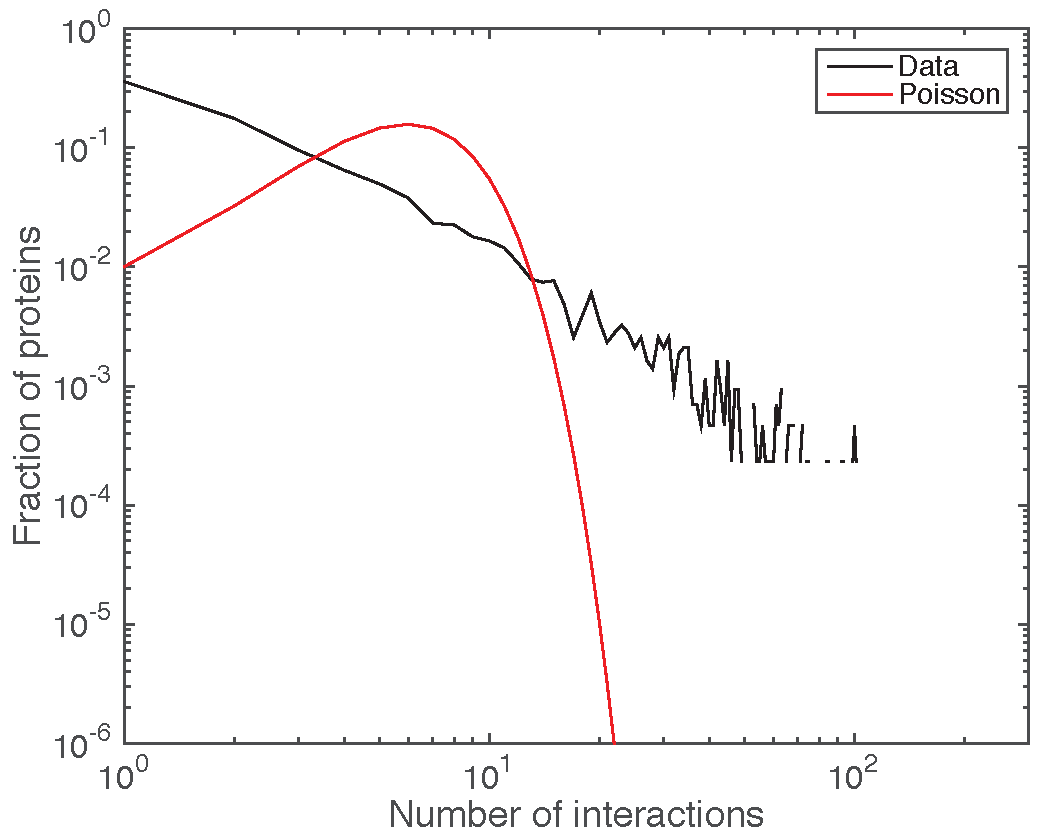
\includegraphics[width=0.4 \textwidth]{prob2c.pdf}\end{center}


\end{enumerate}
An alternative ``preferential attachment" model holds that new edges are connected preferentially to nodes that already have many edges. In the resulting ``scale-free" network, the distribution of edges per node follows a power law.
\begin{enumerate}[a)]
\setlength{\itemsep}{0pt}
\setcounter{enumi}{3}
\item  Fit a power law to the data and plot it on the same axes as in parts (b) and (c). In MATLAB, this can be done with the function \mcode{fit(x,y,'power1')}.\\

\begin{lstlisting}
% Assume that the plot above is still open
power_law_fit = fit(x',y','power1');
plot(power_law_fit,'-b');
legend('Data', 'Poisson', 'Power law','Location','NorthEast')
\end{lstlisting}

\begin{center}
\includegraphics[width=0.4 \textwidth]{prob2d.pdf}\end{center}

\item Which distribution -- Poisson or power law -- is a better fit to the Rolland et al. data? Explain why this distribution may be expected in light of how protein-protein interactions evolve.\\

{\color{red}
The distribution of protein interaction numbers is better fitted by the power law. A few possible explanations:\\

Novel protein-protein interactions may appear randomly by mutation, but those with functional utility are more likely to persist: therefore, it seems unlikely that all possible edges in the protein-protein interaction network occur with equal probability. Preferential attachment is more plausible: consider a protein $X$ which is involved in a critical cellular process and has many binding partners. Since $X$'s function is pivotal, we envision that there are benefits to tightly regulating its activity: adding regulation in the form of e.g. phosphorylation would require acquiring more binding partners from kinases and phosphatases. Conversely, $X$'s tight regulation improves its ability to serve as a regulator of other proteins, allowing $X$ to acquire more targets (another form of binding partners).\\

Answers need not be this detailed and may vary.

}

\item How many self-interactions are reported in this data set? How many self-interactions would you have expected given the number of proteins and the total number of interactions? (You may assume that all edges are equally likely, even if that assumption does not match your results from part e.)

\begin{lstlisting}
disp(sprintf('Detected %d self-interactions; expected %0.2f', self_interactions, m/length(protein_ids)));
\end{lstlisting}

{\color{red}
Expected $13944/4303 = 3.24$ self-interactions; found 517!
}

\item Provide a biological justification for any discrepancy between the two values found in part f.\\

{\color{red}
Many proteins are made up of multiple subunits in which at least two of the subunits are the same. (For example, many transcription factors form homodimers, and hemoglobin forms a dimer of dimers.) This specific form of self-binding likely accounts for the surfeit of self-interactions seen in this data set.
}

\end{enumerate}

\section*{Problem 2: Autorepression with a time delay (50 points)}


In lecture, we studied an autoregulating transcriptional repressor to find its protein abundance $p(t)$ as a function of an input, $x(t)$, that drives the gene's transcription:

\begin{center}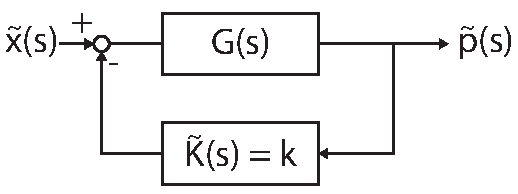
\includegraphics[width=0.4 \textwidth]{autorepression.pdf}\end{center}

We now consider a modified version of this model in which there is a delay $\tau$ between mRNA production and translation\footnote{In eukaryotes, transcriptional elongation, mRNA processing, and nuclear export introduce delays (usually on the order of minutes) between the initiation of transcription and the initiation of translation.}. This delay is reflected in the modified rate equations:
\begin{eqnarray}
\begin{aligned}
\frac{d m}{dt} & = & c_m a(t) - \gamma_m m(t)\\
\frac{d p}{d t} & = & c_p m(t-\tau) - \gamma_p p(t) \label{eqn:rateequations}
\end{aligned}
\end{eqnarray}

\noindent where $a(t)$, the mRNA's net expression level, is $x(t)-k p(t)$ (the activating input minus the strength of the negative autoregulation).

\begin{enumerate}[a)]
\setlength{\itemsep}{0pt}
\item Show using the definition of the Laplace transform that for a function $f(t)$ which is non-zero only for positive $t$,
\[ \mathcal{L}\left[f(t-\tau)\right] = e^{-s\tau} \mathcal{L}\left[f(t)\right] = e^{-s\tau} \tilde{f}(s)\]

{\color{red}
\begin{eqnarray*}
 \mathcal{L}\left[f(t-\tau)\right] & = & \int_0^{\infty} e^{-st} f(t - \tau) \, dt \hspace{1 cm} \textrm{Setting $\sigma = t-\tau$. $d\sigma = dt$:}\\
 & = &  \int_{-\tau}^{\infty} e^{-s(\sigma + \tau)} f(\sigma) \, d\sigma\\
 & = & e^{-s\tau} \int_0^{\infty} e^{-s \sigma} f(\sigma) \, d\sigma\\
 & = & e^{-s\tau} \tilde{f}(s)
\end{eqnarray*}

}

\item Transform rate equations (\ref{eqn:rateequations}) and simplify to find an expression for the forward transfer \linebreak  function $G(s) =\tilde{p}(s)/\tilde{a}(s)$. Assume that $m(0)=p(0)=0$.\\

{\color{red}
\begin{eqnarray*}
s \tilde{m}(s) - m(0) = s \tilde{m}(s) & = & c_m \tilde{a}(s) - \gamma_m \tilde{m}(s)\\
\tilde{m}(s) & = & \frac{c_m \tilde{a}(s)}{s + \gamma_m}\\
s \tilde{p}(s) - p(0) = s \tilde{p}(s) & = & c_p e^{-s\tau} \tilde{m}(s) - \gamma_p \tilde{p}(s)\\
\tilde{p}(s) & = & \frac{c_p e^{-s\tau} \tilde{m}(s)}{s + \gamma_p} = \frac{c_m c_p \tilde{a}(s)}{(s + \gamma_m)(s+\gamma_p)} \\
G(s) = \frac{\tilde{p}(s)}{\tilde{a}(s)} & = & \frac{c_m c_pe^{-s\tau}}{(s + \gamma_m)(s+\gamma_p)} 
\end{eqnarray*}
}

\item Find an expression for the closed loop transfer function $\tilde{p}(s)/\tilde{x}(s)$ in terms of $k$ and $G(s)$.\\


{\color{red}

The input to the plant is $\tilde{a}(s) = \tilde{x}(s) - k \tilde{p}(s)$. The output from the plant is:
\begin{eqnarray*}
\tilde{p}(s) & = & G(s) \tilde{a}(s) = G(s)  \tilde{x}(s) - k G(s) \tilde{p}(s)\\
\left[ 1 + k G(s) \right] \tilde{p}(s) & = & G(s)  \tilde{x}(s)\\
\textrm{Closed loop transfer function } \frac{\tilde{p}(s)}{\tilde{x}(s)} & = & \frac{G(s)}{1+kG(s)}
\end{eqnarray*}
}

\end{enumerate}
The autorepression system is unstable if any poles of the closed loop transfer function have a positive real part.
\begin{enumerate}[a)]
\setlength{\itemsep}{0pt}
\setcounter{enumi}{3}
\item Show that the only poles of the closed loop transfer function which could have a positive real part are the roots of $1 + kG(s)$.\\

{\color{red}

A point $s$ is a pole of the closed loop transfer function if:
\begin{enumerate}[i)]
\item $s$ is a pole of the numerator, $G(s)$
\item $s$ is a zero (also called a root) of the denominator, $1+kG(s)$
\end{enumerate}

The only poles of $G(s)$ are $s=-\gamma_m$ and $s=-\gamma_p$, where are both real and negative. Therefore, if any poles of the closed loop transfer function have a positive real part, they must be roots of $1+kG(s)$.
}

\end{enumerate}
The result in part (d) implies that the system will be unstable if any roots of $1 + kG(s)$ have a positive real part. The Nyquist stability criterion can be used to determine whether any such roots exist, but in order to apply it, we must first know the number of poles of $1 + kG(s)$ with a positive real part.
\begin{enumerate}[a)]
\setlength{\itemsep}{0pt}
\setcounter{enumi}{4}
\item Demonstrate that the number of poles of $1 + kG(s)$ with positive real part is zero.\\

{\color{red}
Plugging in our solution for $G(s)$:
\[ 1 + k G(s) = \frac{(s + \gamma_m)(s+\gamma_p)}{(s + \gamma_m)(s+\gamma_p)} + \frac{kc_m c_pe^{-s\tau}}{(s + \gamma_m)(s+\gamma_p)}  = \frac{(s + \gamma_m)(s+\gamma_p) + k c_m c_pe^{-s\tau}}{(s + \gamma_m)(s+\gamma_p)} \]

We can see by examination that the only roots of $1+kG(s)$ are $s=-\gamma_m$ and $s=-\gamma_p$, where are both real and negative. Therefore, $P=0$.

}
\end{enumerate}
The absence of poles with positive real part implies that the number of zeros of $1 + kG(s)$ with positive real part is equal to the number of times that the Nyquist plot of $1 + kG(s)$ encloses the origin clockwise. Equivalently, the system is stable if the Nyquist plot of $G(s)$ does not enclose the point $-1/k$.

\begin{enumerate}[a)]
\setlength{\itemsep}{0pt}
\setcounter{enumi}{5}
\item Show that $G(s) \to 0$ as $|s| \to \infty$. [The Nyquist plot is therefore well approximated by $G(s=i\omega)$ for $\omega \in (-n, n)$ with sufficiently large $n$: we can ignore other points on the Nyquist contour.]\\

{\color{red}
Let $s = a + bi$ lie outside the left half plane ($a \geq 0$), as it must for any point on the arc of the Nyquist contour. Consider the numerator of $G(s)$:

\begin{eqnarray*}
c_m c_p e^{-\tau (a + bi)} & = & c_m c_p e^{-\tau a } e^{- \tau bi} 
\end{eqnarray*}

Since $\tau$ and $a$ are non-negative, $0 < e^{-\tau a} \leq 1$. The sinusoidal component is likewise bounded: $-1 \leq e^{-\tau bi} \leq 1$. Therefore the numerator of $G(s)$ is bounded within $[-c_m c_p, c_m c_p]$.\\

As for the denominator of $G(s)$,

\begin{eqnarray*}
\left(s + \gamma_m \right) \left(s + \gamma_p \right) & = & \left(a + \gamma_m + bi \right) \left(a + \gamma_p + bi \right)\\
& = & \left(a + \gamma_m \right) \left( a + \gamma_p \right) - b^2 + bi \left(2a + \gamma_m + \gamma_p \right)
\end{eqnarray*}

Since at least one of $a$ and $b$ must be infinite for all points on the arc ($|s| \to \infty$, $a > 0$), it is clear that the magnitude of the denominator of $G(s) \to \infty$ as $|s| \to \infty$. Since the numerator is bounded, this implies that $G(s) \to 0$ and $|s| \to \infty$.

}


\item Use MATLAB to plot $G(i\omega)$ on the complex plane for $\omega \in (-100, 100)$. Use $c_i=\gamma_i=1$ and two values of $\tau$: 0 and 1.

\begin{lstlisting}
function [] = nyquist_delay()
    tau = 0;
    F = @(w) exp(- i .* w .* tau)./((i.*w+1).*(i.*w+1));
    w = linspace(-100, 100, 100000);
    result = F(w);
    plot(real(result(:)), imag(result(:)), '-r'); hold on;
    
    tau = 1;
    F = @(w) exp(- i .* w .* tau)./((i.*w+1).*(i.*w+1));
    result = F(w);
    plot(real(result(:)), imag(result(:)), '-b');
    xlabel('Real')
    ylabel('Imaginary')
    legend('\tau=0','\tau=1','Location','NorthEast')
    set(gca, 'FontSize', 16)
end
\end{lstlisting}

\begin{center}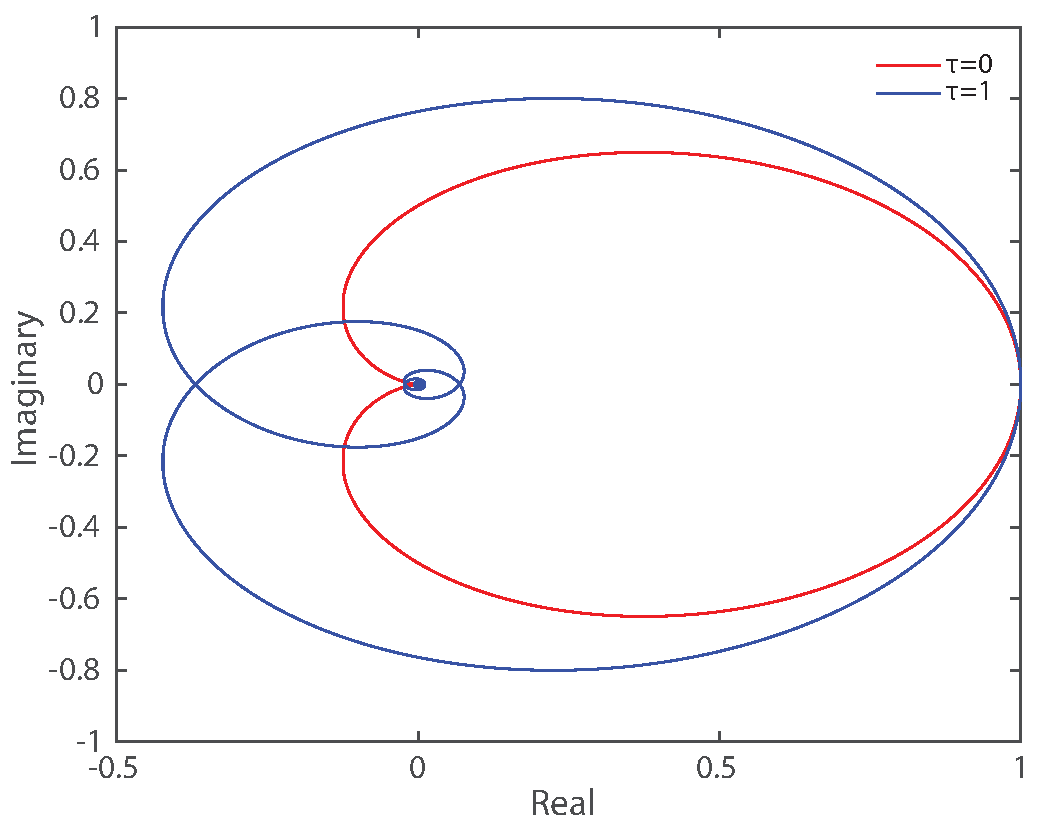
\includegraphics[width=0.5 \textwidth]{nyquist.pdf}\end{center}

{\color{red}
Note: another option would've been to simply plug in $\tau$ and the other constants, then create a transfer function using MATLAB's \mcode{tf()} and \mcode{nyquist()}.

}

\item Show using your $\tau=1$ Nyquist plot that there exists a threshold gain $k^*$ above which the system is unstable. (Though you will not show it explicitly, this is true for all $\tau,c_i, \gamma_i>0$.) Confirm from the $\tau=0$ Nyquist plot that the system is stable for all $k$ when there is no time delay.\\

{\color{red}
When $\tau=1$, the Nyquist plot of $G(s)$ encircles a range of points on the negative real axis: $(-1/e,0)$. This means that the system is unstable if $k>k^*=e$.\\

When $\tau=0$, no points on the negative real axis are enclosed, so there is no threshold gain value $k^*$ above which the system is unstable.
}

\item Approximately what value of the repressor's gain $k$ would be ideal when $\tau=c_i=\gamma_i=1$? (That is, what value of $k$ minimizes the deviation of $p(t)$ from zero in this case?)\\

{\color{red}
The gain should be chosen as high as possible to minimize droop without causing the system to become unstable. There, we choose $k$ only slightly below the threshold, $k^*=1/e$.

}

\item The repressor's gain $k$ can be adjusted through mutation and natural selection. Describe two types of mutations that could alter the value of $k$.\\

{\color{red}

Higher gain corresponds to stronger self-regulation of the repressor. This could be altered by mutating the repressor's binding site in its own promoter to either strengthen or weaken its effective binding constant. Alternatively, the repressor's DNA binding domain amino acid sequence could be mutated, affecting the strength with which the protein can bind to its site in its own promoter.

}
\end{enumerate}

\end{document}